\documentclass[12pt]{article}

\usepackage{sbc-template}

\usepackage{graphicx,url}

%\usepackage[brazil]{babel}   
\usepackage[utf8]{inputenc}  

     
\sloppy

\title{Travelling Salesperson Problem:\\ Different Approaches and Performance in Exponential Time}

\author{Juan M. Braga F.\inst{1}}


\address{Departamento de Ciência da Computação -- Universidade Federal de Minas Gerais
  (UFMG)\\
  Av. Pres. Antônio Carlos, 6627 -- Pampulha -- Belo Horizonte -- MG -- Brazil
  \email{juanbraga@ufmg.br}
}

\begin{document} 

\maketitle

\begin{abstract}
  This paper documents the practical aspects of implementing solutions
  for the Travelling Salesperson Problem, a well known difficult problem that requires
  exponential time for the optimal solution. Three algorithms were implemented:
  an exact solution through the branch-and-bound technique, and two other approximations,
  the twice-around-the-tree and Christofides algorithms.
\end{abstract}
     
\begin{resumo} 
  Este artigo documenta os aspectos práticos da implementação de soluções
  para o Problema do Caixeiro Viajante, um problema bem conhecido e difícil que requer
  tempo exponencial para encontrar a solução ótima. Foram implementados três algoritmos:
  uma solução exata através da técnica de branch-and-bound, e duas outras aproximações,
  os algoritmos twice-around-the-tree e Christofides.
\end{resumo}


\section{Introducing the Travelling Salesperson Problem}

The Travelling Salesperson Problem (TSP) is aptly described by \cite{brilliant_explanation} 

\begin{quote}
  "A salesperson needs to visit a set of cities to sell their goods. They know how 
  many cities they need to go to and the distances between each city. In what order 
  should the salesperson visit each city exactly once so that they minimize their 
  travel time and so that they end their journey in their city of origin?"
\end{quote}

The TSP is a well known \textbf{intractable problem}, which in the context of 
algorithms means that the time and/or space required to solve the problem grows 
exponentially with the size of the input, making it impractical to solve even for 
relatively small inputs.

This project documents the development of three solutions for the given problem, 
focusing on evaluating the real-world challenges associated with them, such as planning and 
optimization, making informed decisions on data structures and libraries, and 
analyzing the usage of computer resources.

\section{Modelling and Implementation}

The TSP problem can be conveniently modeled by a weighted graph, with the graph's 
nodes representing the cities and the edge weights specifying the distances.

To solve it, three algorithms were implemented in this project: an optimal solution using 
the branch-and-bound technique, and two approximations, the twice-around-the-tree and the 
Christofides algorithms.

\subsection{Optimal Solution}

Branch and bound is a general method that tries to divide a problem into smaller subproblems,
and then makes informed decisions to discard some of these subproblems to reach the optimal solution.

To consider it in the TSP context, one benefits from \textbf{picturing the problem as a tree}, where each node 
represents a city and each edge a path between two cities. Then, the first node can be any city 
(since one can start from any city of the optimal path without changing the path distance), and 
the path from the origin node to a leaf in the graph should represent the total 
lengh of that path.

However, simply storing the entire tree will evidently yield an enormous amount 
of data, as all possible combinations would end up stored in memory. That is why the 
branch and bound technique must make the decision of which city to visit next based 
on all of the previous decisions, which can be called a \textbf{lower bound}.

The lower bound parameter for selecting the next city is calculated by summing the 
distance of the current path with the minimum distance to any unvisited city. By 
maintaining this metric for each partial path, the branch and bound algorithm 
discards subproblems that cannot possibly lead to the optimal solution, effectively 
focusing on the most promising paths.

[TODO START COST ESTIMATE]

\subsection{Approximate Solution: Christofides}

The Christofides algorithm was built by leveraging a key insight: many of the edges on the 
optimal solution are often found on the Minimmum Spanning Tree (MST) of the same graph 
\footnote{\cite{reducible_explanation}}. Therefore, as there are known relativelly efficient 
algorithms for generating the MST, it makes sense to try and make use of this fact.

To form an optimal solution, all nodes of the MST should have an even number of edges, so 
that the salesperson could enter and leave the city through exactly two edges (also known as an 
\textit{Eulerian Tour}). However, most MSTs have nodes with an odd number of edges, 
which will require more edges to be added.

The second part of the solution involves finding good edge candidates to append to te odd 
edges. Out of multiple available options, the approach used in this implementation was the minimun-length
matching of the odd-degree nodes, which tries to find a maximum matching in a bipartite 
graph with minimum total weight. In other words, it tries to find the best nodes (shortest distance) 
that connect every pair of the odd-degree nodes of the MST.

Combining the MST with the minimum-length matching will provide us with a very good 
approximation of the TSP's optimal solution, which can be easily constructed by
traversing this graph while taking shortcuts to avoid visiting multiple cities.

According to \cite{Johnson2003}, the Christofides algorithm provides a better 
worst-case guarantee than any other currently known tour construction heuristic: a worst case ratio of 1.5; 
[and] it also tends to find better tours in practice. However, [C]omputing the minimum-length 
matching on the odd-degree vertices remains the bottleneck of the algorithm.

\subsection{Approximate Solution: Twice Around the Tree}

[TODO DESCRIPTION OF TWICE-AROUND-THE-TREE]
[guarantee of 2 of optimal solution]

\subsection{Implementation Choices}

The programming language used was Python 3.12, and the program was executed 
in a Python Virtual Environment on the Ubuntu 23.10 Linux distribution, on a computer with a 
Intel Core i5-4690K processor and 8GB of RAM at 2133MHz.

The \textbf{datasets} were selected by the professor from the TSPLIB \cite{datasets_lib}. They are 
composed of \texttt{.tsp} files with the node key and its $x$ and $y$ location in the carthesian plane. 
The graphs are to be constructed by considering that all cities are connected to all other cities, forming 
a totally connected graph.

The chosen \textbf{data structure} for the approximate algorithms was the graph implementation 
by the \texttt{networkx} library in python \cite{networkx_docs}, as recommended by 
the professor in the project specifications. To prevent excessive use of Python loops, 
the internal \texttt{networkx} functions were also used, such as \texttt{minimum\_spanning\_tree} , 
\texttt{eulerian\_circuit} and \texttt{min\_weight\_matching}.

The \textbf{libraries} \texttt{time} and \texttt{memory\_profiler} were chosen to keep track of time 
and allocated memory, as they provided the most convenient interface. It must be noted that the library 
to monitor the memory gives a significant increase in memory use, so the implementation allowed for 
two executions: one for testing time and performance and another to keep track of the memory.

\textbf{Execution Instructions:}
- Make sure that a compatible Python version and the libraries used (See above) are installed.
- Select the desired datasets to be used in the \texttt{dataset_schema.txt} file.
- Make sure the respecive dataset \texttt{.tsp} files are in the \texttt{datasets/} subfolder.
- Choose which algorithm will be run and wether to skip memory monitoring in the \texttt{main.py} file.
- Run the code in a terminal with the following command: \texttt{python main.py} or \texttt{python3 main.py}.
- The results will be located on a file called \texttt{statistics.csv}.

\section{Experiments} \label{sec:firstpage}
    Apresentar os experimentos e discutir os resultados. Você deve avaliar os
    limites de cada algoritmo/implementação, tentando buscar uma relação entre
    tamanho da instância e desempenho. Deve também comparar os algoritmos
    entre si. Tente responder quando cada implementação se sai melhor ou
    deveria ser usada.

The qualities of each algorithm will be evaluated through four metrics: the time elapsed 
to find the solution, the amount of memory used and the quality of the solutions found 
compared to the optimal solution (see [TODO SECTION IMPLEMENTATION CITE] for information 
on libraries used).

\subsecion{Memory Use}

The first and most important aspect when dealing with exponential optimisation algorithms such as 
the TSP is the use of memory. In order to make informed decisions about all possible combinations, 
it is often necessary to store information about many or all of the previous decisions, not to 
mention storing the entire problem.

For this project, the chosen data structure implementation (See [TODO REFERENCE]) works by storing 
the entire graph in memory, so simply storing the dataset is the first memory bottleneck.

For the 

\begin{figure}[ht]
\centering
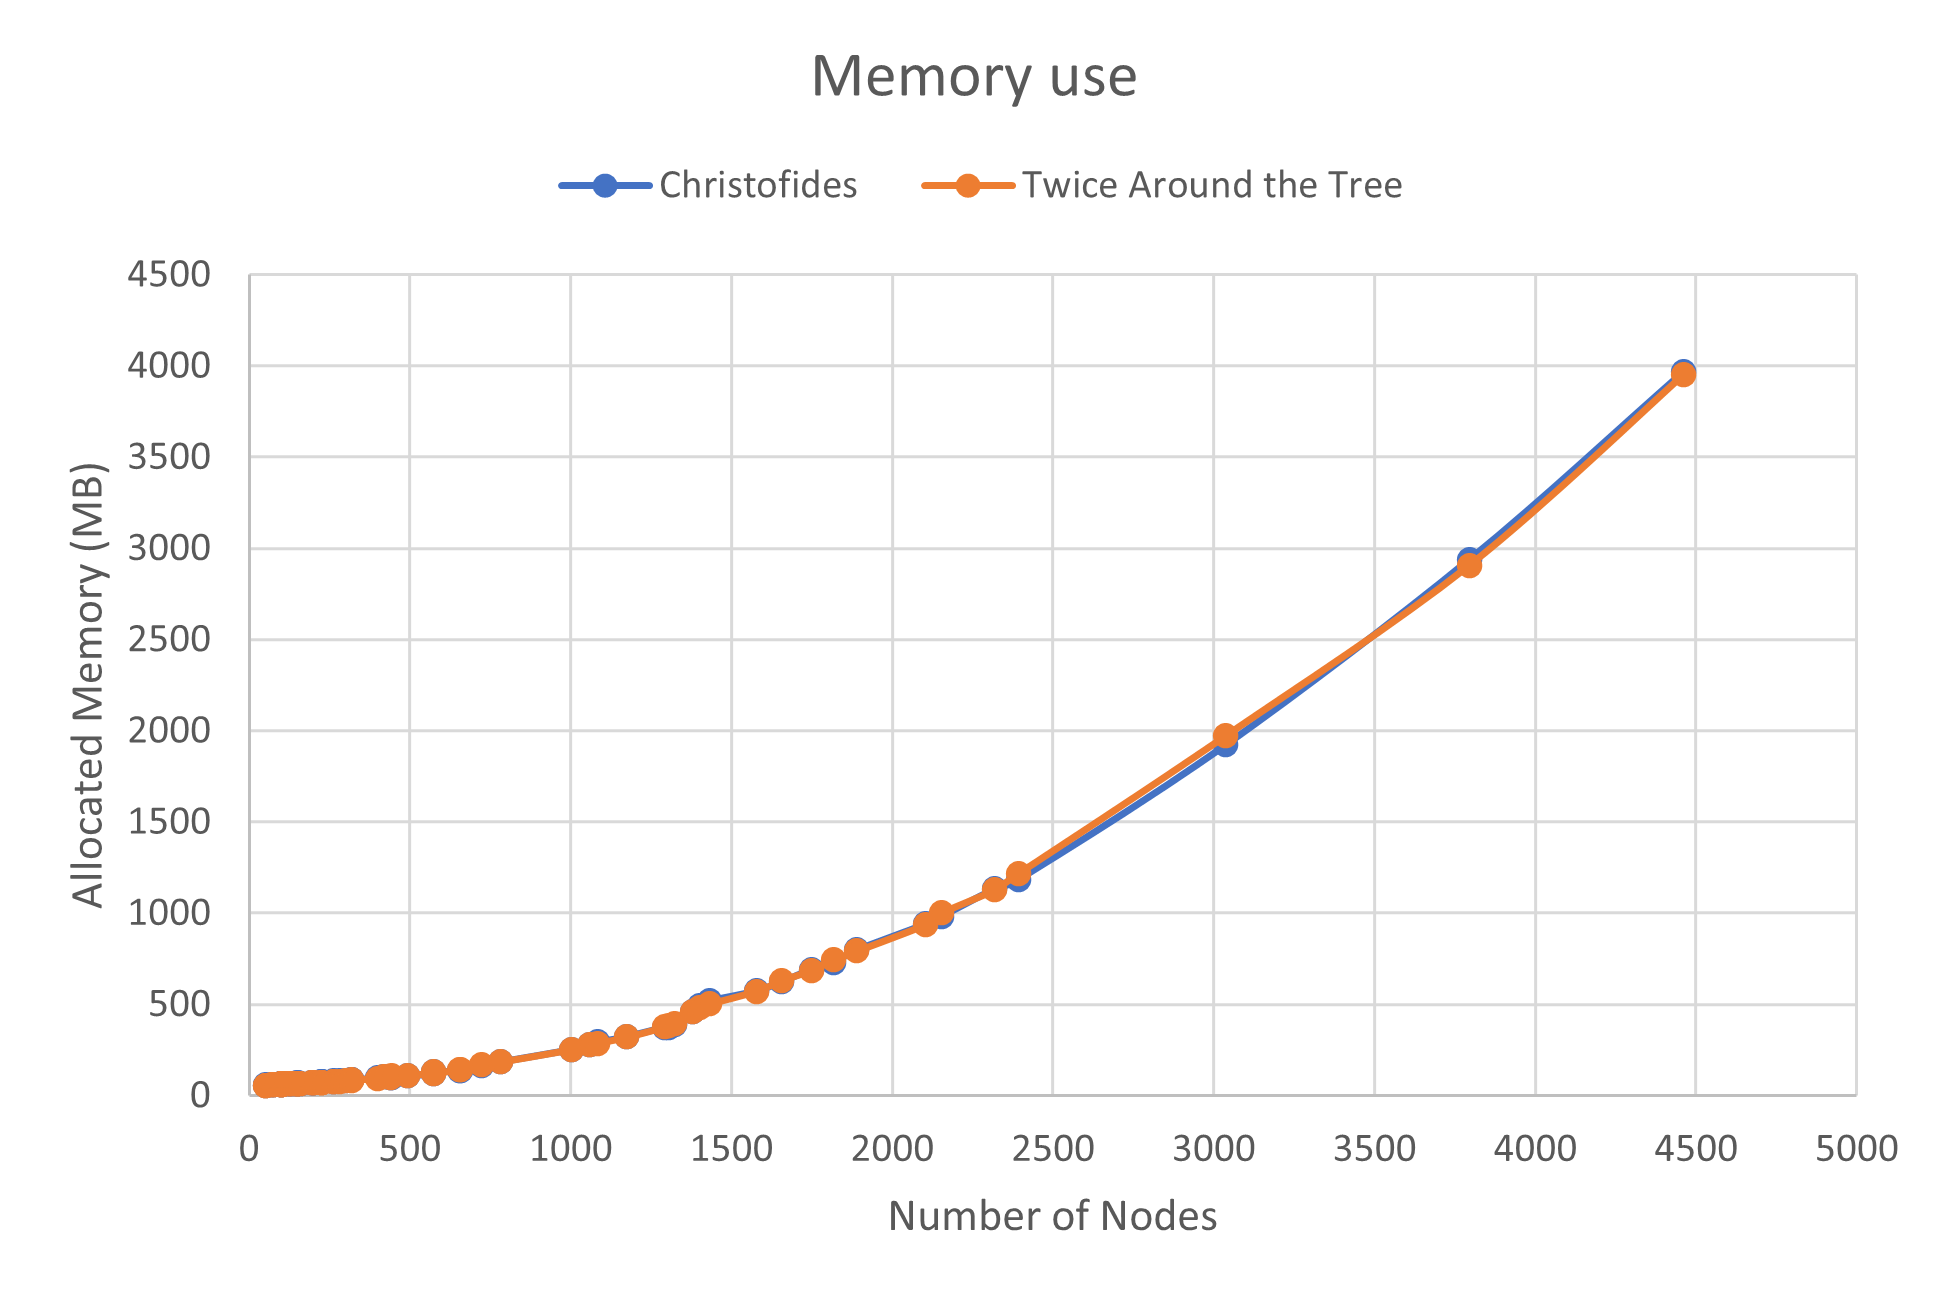
\includegraphics[height=.325\textheight]{memory_use_comparison.png}
\caption{Chart comparing the allocated memory between the Christofides and the Twice-around-the-tree algorithms.}
\label{fig:mem_use}
\end{figure}

starting with the datasets with 3795 cities (fl3795) for the Christofides algorithm, 
and with [TODO NUMBER] cities ([TODO DATASET]) for the Twice-around-the-tree, the the allocated memory did surpass 
the available RAM capacity ([TODO REFERENCE SECTION WITH MEMORY]) and storage in the \texttt{swap}/\texttt{paging} 
file 
\footnote{Swap or Page file is a section of a hard drive used as a temporary location to store information 
when the computer's RAM (random-access memory) is fully utilized. It has significantly slower speeds when 
compared with the primary memory.} 
was triggered.

Datasets starting with [TODO] cities for the Twice-around-the-tree and with [TODO] for the Christofides were 
not even able to be stored in the available memory and caused the computer to crash.


\subsection{Solution Quality}

The graph of the Figure~\ref{fig:quality_ratio} shows the ratio \frac{Approximate Solution}{Optimial Solution}.

\begin{figure}[ht]
\centering
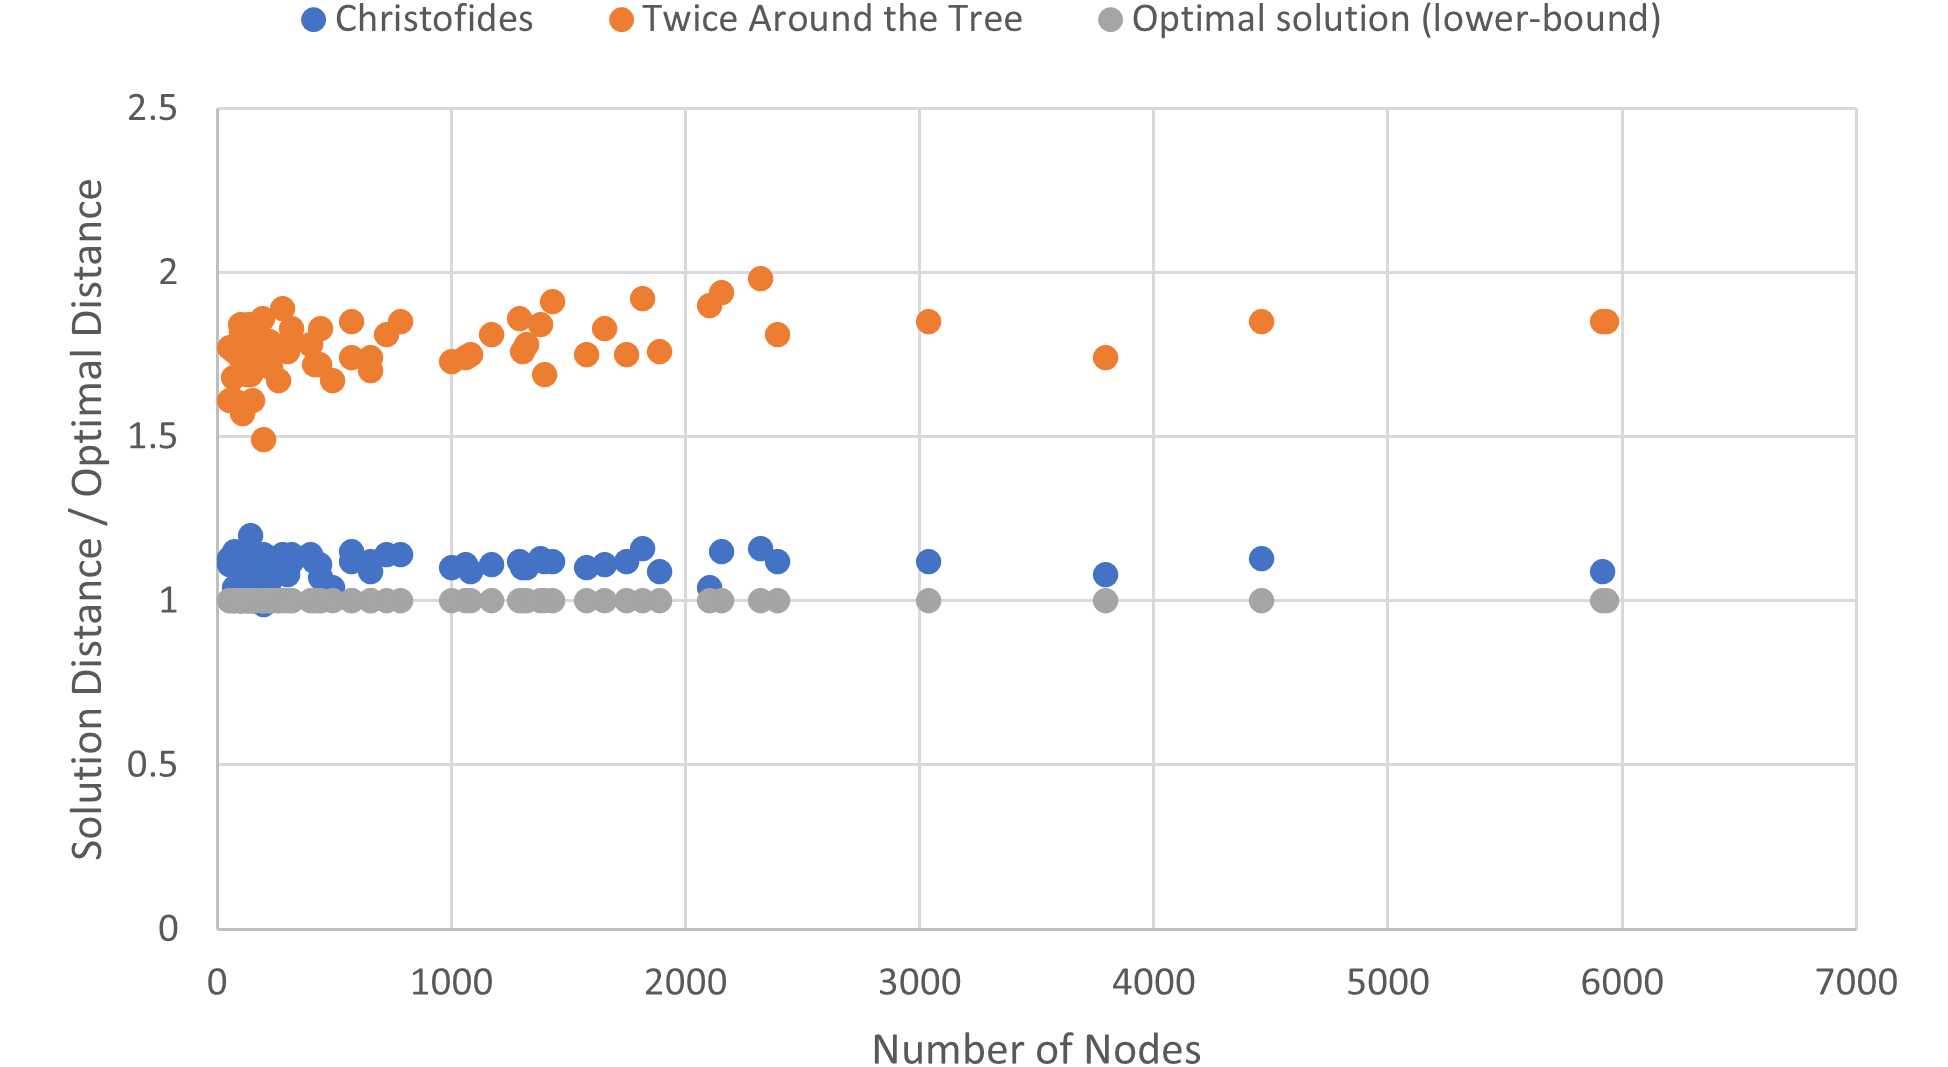
\includegraphics[height=.325\textheight]{quality_ratio.png}
\caption{Chart comparing the quality of the approximate and optimal solutions.}
\label{fig:quality_ratio}
\end{figure}

The Twice-around-the-tree stays consistently below the expected theoretical worst case ([TODO SEE SECTION]) of 
twice the optimal solution, and the Christofides solutions find paths that are consistently better and closer to it, 
also keeping the tight 1.5 quality ratio.

\subsection{Execution Time}

The execution time of the algorithms can be compared with the following Figure~\ref{fig:exec_time}.

\begin{figure}[ht]
\centering
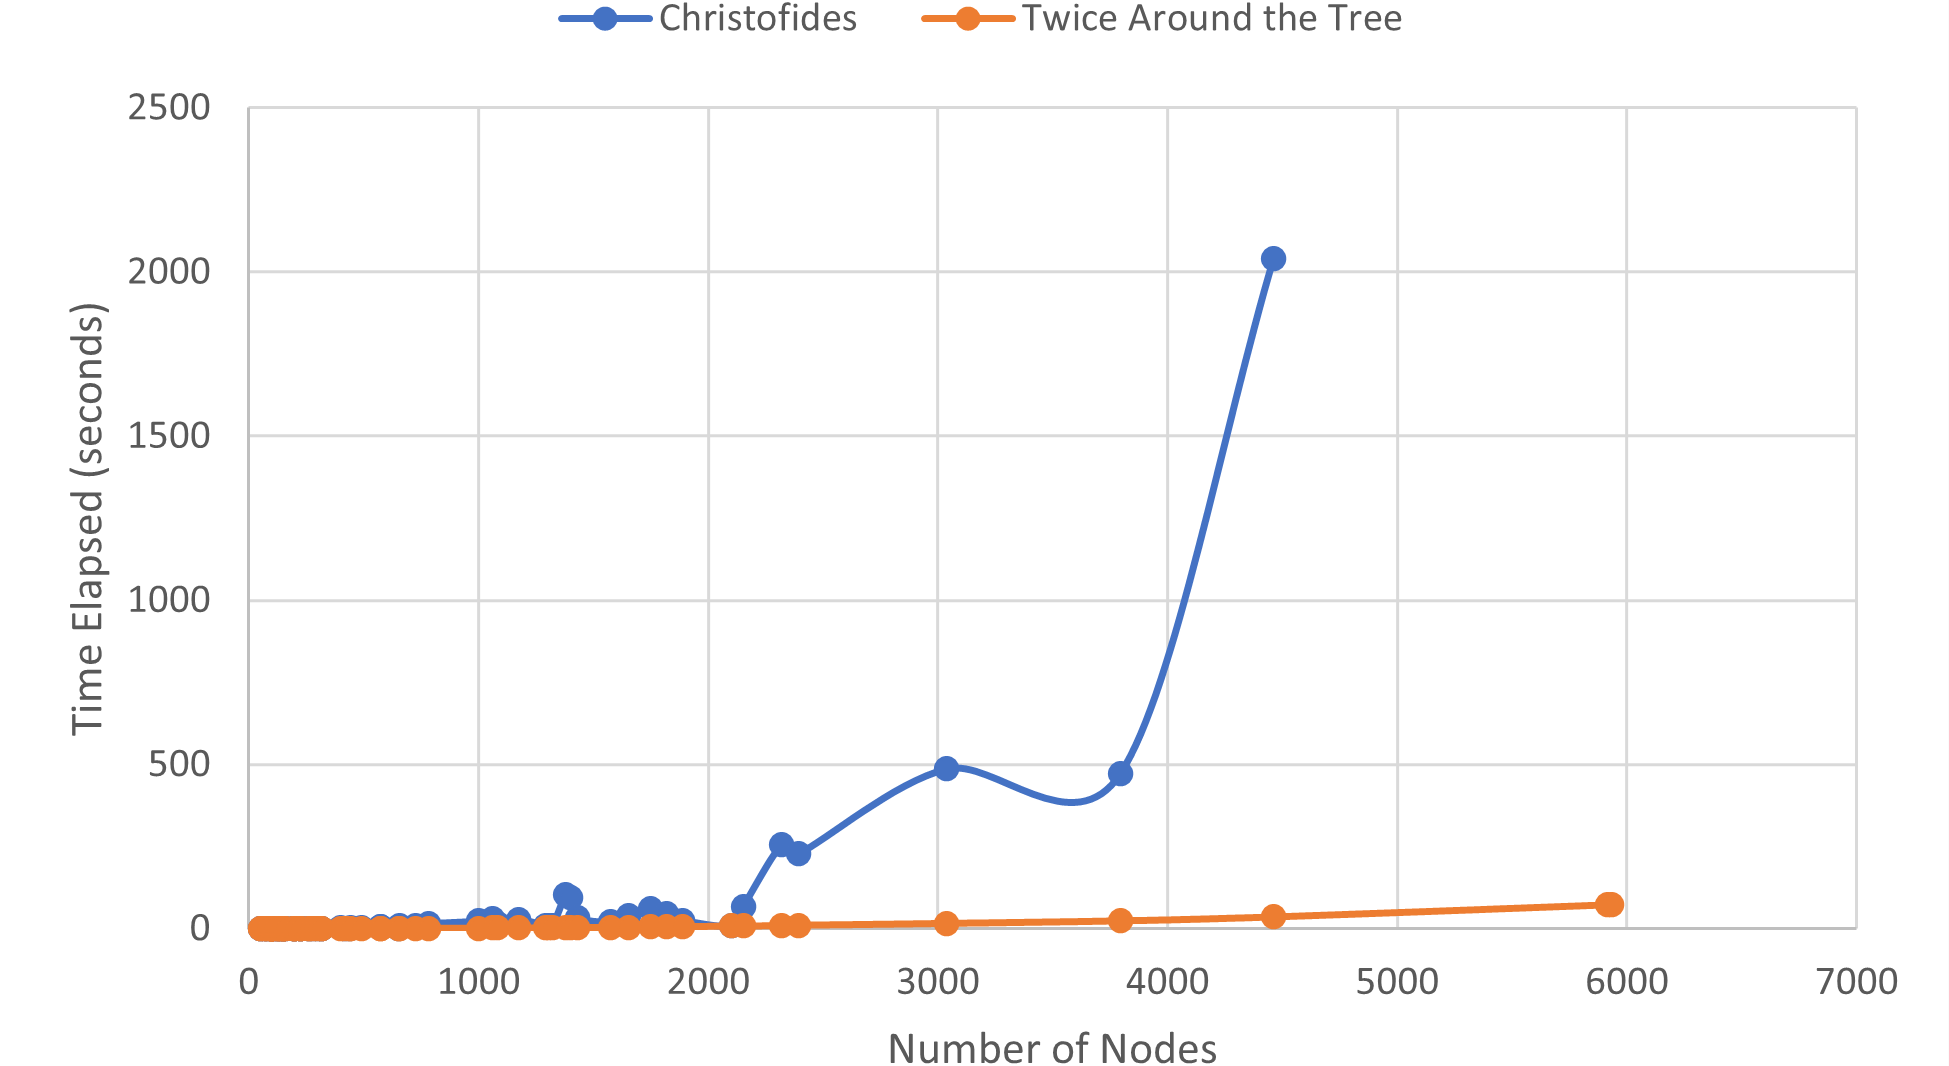
\includegraphics[height=.325\textheight]{execution_time_comparison.png}
\caption{Chart comparing the time elapsed between the Christofides and the Twice-around-the-tree algorithms.}
\label{fig:exec_time}
\end{figure}

The Christofides algorithm takes significantly longer to run when compared to the Twice-arount-the-tree. 
In fact, it appears to form an exponential growth, but that must be put into perspective as the student 
has diagnosed that the algorithms exceeded the available RAM memory (See [TODO SECTION]), and therefore 
the graph does not display their ideal behviour (suffering from the slow speeds of the swap/paging memory).

The use of the \texttt{swap} therefore indicates that the time data does not perfectly represent the ideal behaviour 
of the algorithms, and perfectly illustrates how difficult it is to optimise exponential algorithms for relatively 
small cases. [TODO REFER SECTION ON MEMORY]

\section{Conclusions}
    Apresente as conclusões do seu trabalho. Mostre o quê pôde ser percebido
    com seus experimentos.

\bibliographystyle{sbc}
\bibliography{sbc-template}

\end{document}
